% !TEX root = ../../技术文档.tex
\section{特性成果}

\subsection{CPU性能}

CPU性能采用CoreMark 1.0\cite{eembc-coremark-rules}，按发射宽度和存储路径分别记录板测结果。双发射与单发射均列出本地SRAM和L1 Cache＋板载DDR两类配置。

双发射板测采用六级RV32IM/Zicsr核，分别连接32\,KiB片上SRAM和L1 Cache＋板载DDR。
SRAM配置将程序、数据及栈放在本地存储，关闭Cache；DDR配置将程序、数据及栈放在私有DDR区，经各16\,KiB的I/D Cache访问。
CPU标称频率为100\,MHz，编译器为GCC 15.2.0，使用\texttt{-march=rv32im\_zicsr}、\texttt{-mabi=ilp32}和\texttt{-O2}，不启用LTO；CoreMark执行5000次迭代。
两组结果见表\ref{tbl:cpu-dual-coremark}，两者均通过标准CRC检查，\texttt{errors=0}、\texttt{short=0}且输出\texttt{CPU\_COREMARK\_BOARD\_PASS}。

\begin{reporttable}
\begin{longtable}{@{}p{0.30\linewidth}p{0.32\linewidth}p{0.32\linewidth}@{}}
\caption{双发射CPU板级CoreMark结果}\label{tbl:cpu-dual-coremark}\\
\toprule
项目 & TCM & L1 Cache＋板载DDR \\
\midrule
\endfirsthead
\caption[]{双发射CPU板级CoreMark结果（续）}\\
\toprule
项目 & TCM & L1 Cache＋板载DDR \\
\midrule
\endhead
\bottomrule
\endfoot
发射宽度 & 2 & 2 \\
CPU标称频率 & 100\,MHz & 100\,MHz \\
迭代次数 & 5000 & 5000 \\
计时区间周期数 & 1,221,660,558 & 1,586,210,467 \\
运行时长 & 12.21660558\,s & 15.86210467\,s \\
CoreMark & 409.278990 & 315.216681 \\
CoreMark/MHz & 4.092789 & 3.152166 \\
CPU核占用LUT & 9677 & 9707 \\
CoreMark/LUT & 0.042293 & 0.032473 \\
\end{longtable}
\end{reporttable}

运行时长由完整周期数除以100\,MHz计算，CoreMark为5000次迭代除以运行时长，CoreMark/MHz再除以100，CoreMark/LUT除以对应CPU核LUT数。
表中分数保留串口输出的六位小数，其输出方式为截断；运行时长按完整周期数列出，不使用整数秒对应的Iterations/Sec字段。
SRAM的本地访问延迟较低，Cache＋DDR配置还包含缓存查询、未命中填充及外部存储等待，两者分别描述对应存储路径下的板级性能。

图\ref{fig:cpu-dual-coremark-uart}并列展示两组完整串口原始截图，保留配置、编译参数、计时、评分和校验信息。
原图及配置、资源、时序证据索引见\path{docs/verification/cpu/report_configurable_issue_2026-11-02/}。

\begin{figure}[!htbp]
\centering
\makebox[0.49\linewidth][c]{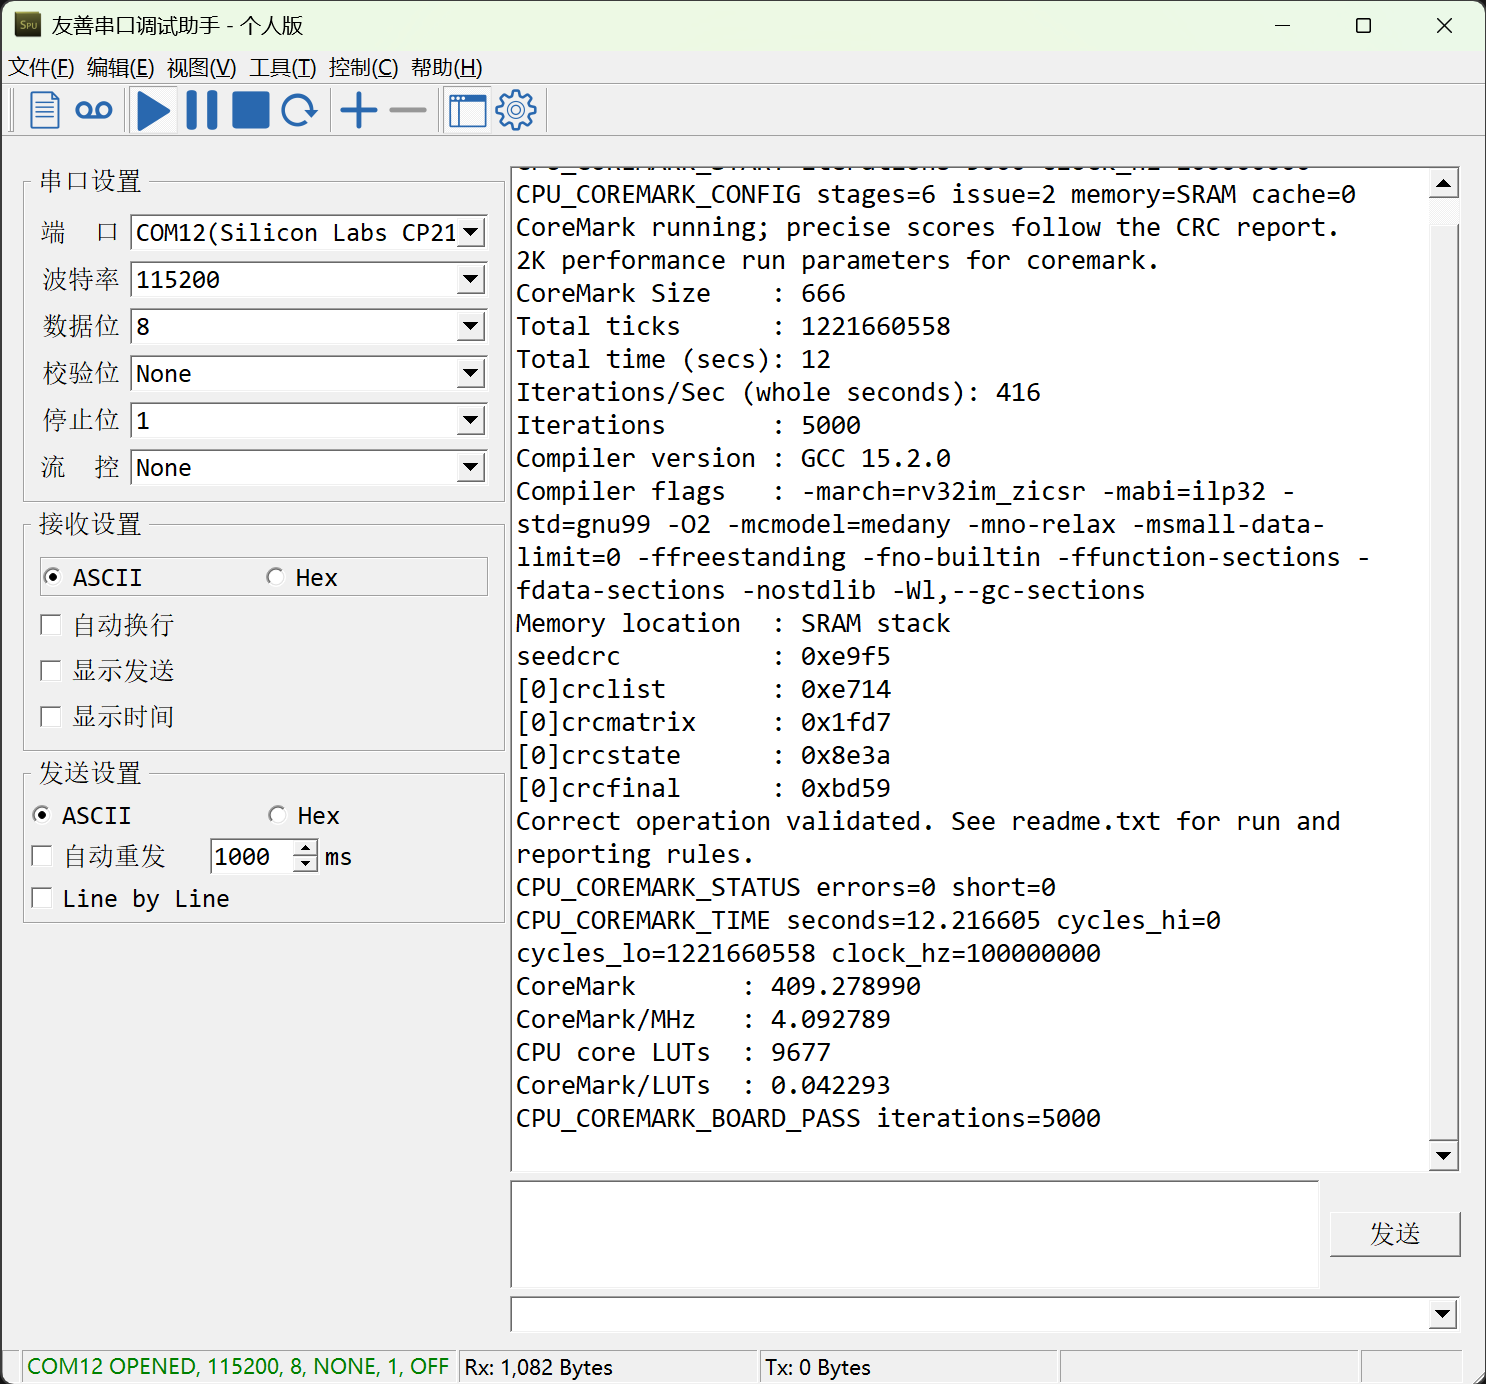
\includegraphics[height=0.41\linewidth]{../figure/cpu-dualissue-sram-coremark-uart-original.png}}\hfill
\makebox[0.49\linewidth][c]{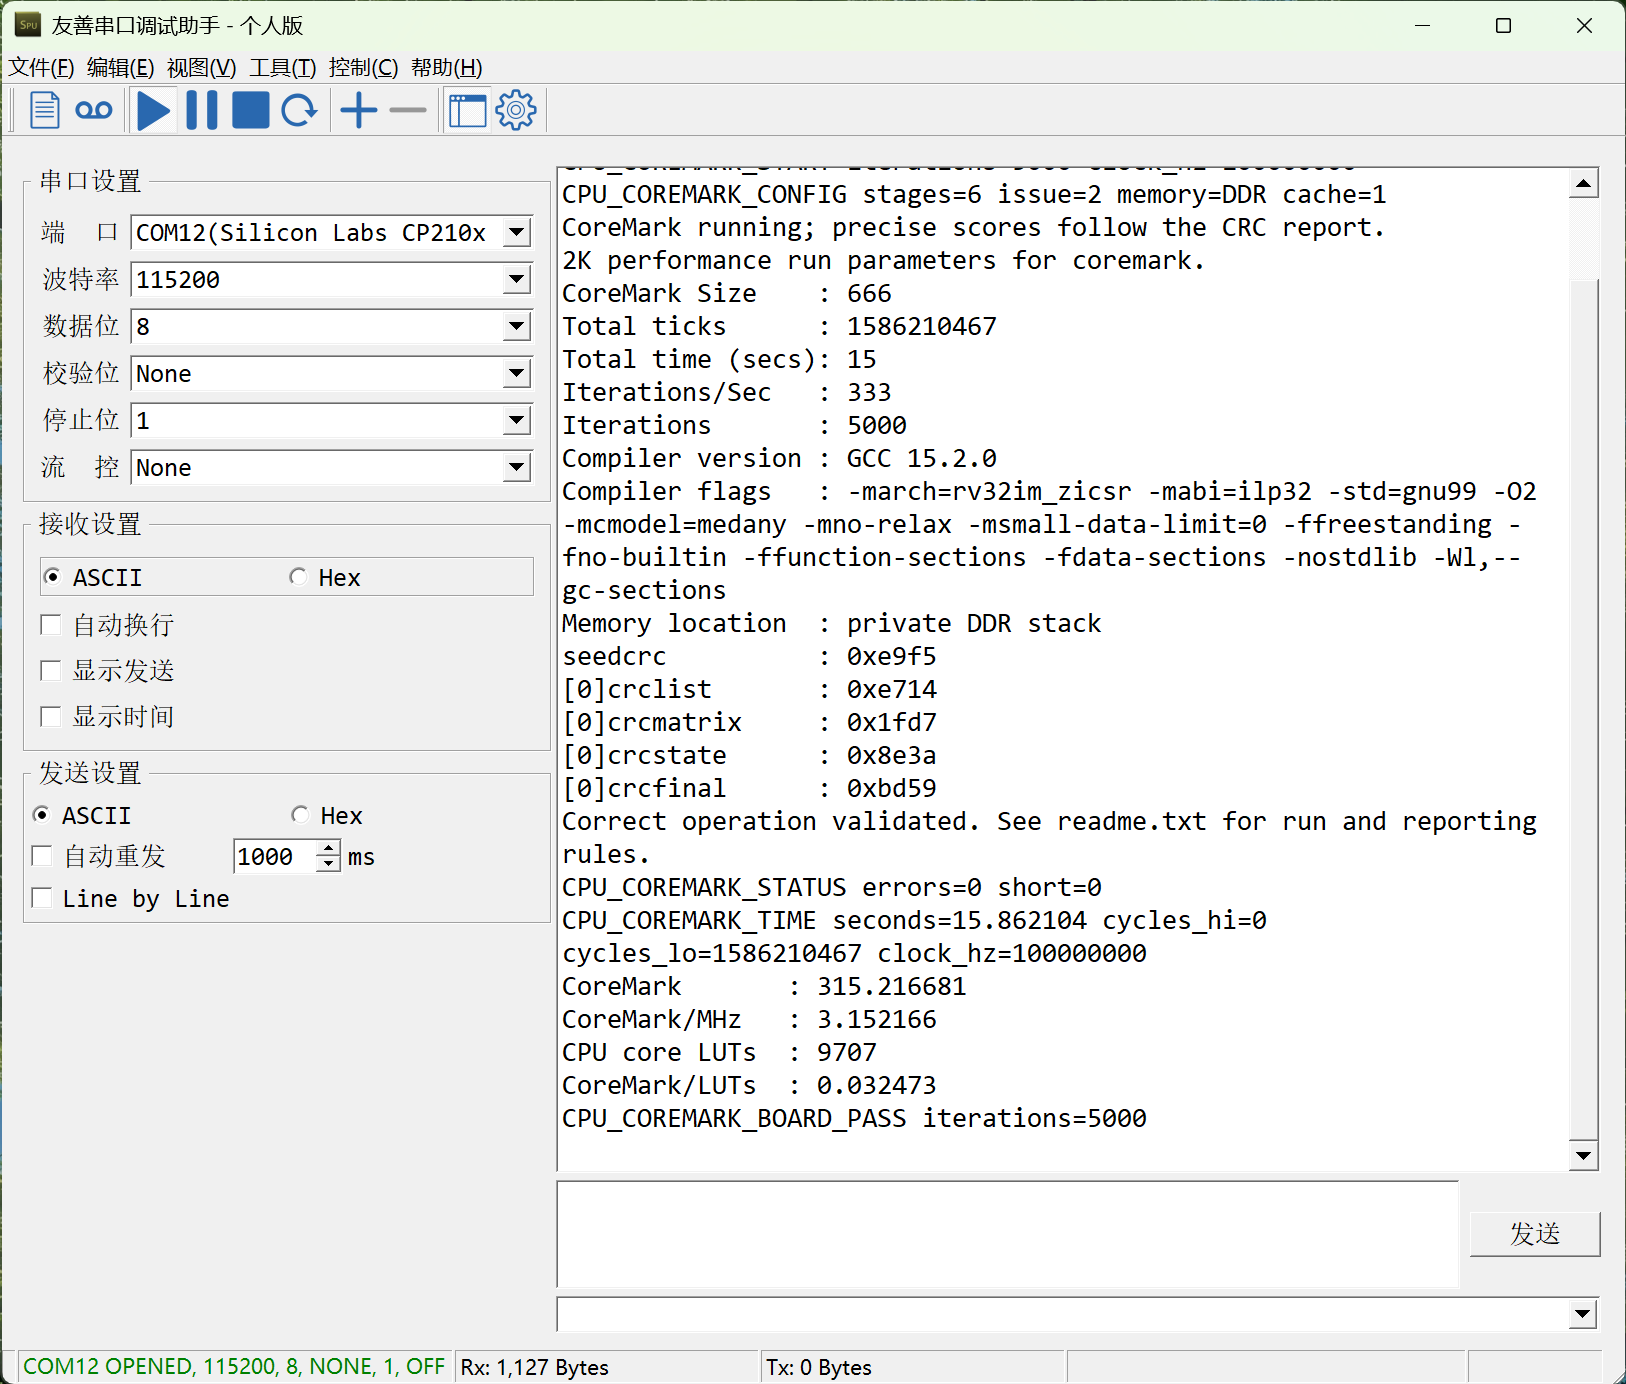
\includegraphics[height=0.41\linewidth]{../figure/cpu-dualissue-cache-ddr-coremark-uart-original.png}}
\par\smallskip
\makebox[0.49\linewidth][c]{\small (a) SRAM，Cache关闭}\hfill
\makebox[0.49\linewidth][c]{\small (b) L1 Cache＋板载DDR}
\caption{双发射CPU两种存储配置的CoreMark完整串口截图}\label{fig:cpu-dual-coremark-uart}
\end{figure}

单发射板测分别采用TCM本地存储和L1 Cache配合板载DDR。
TCM由直接连接CPU本地访问路径的32\,KiB片上SRAM实现，程序、工作数据和栈均驻留其中，不经过I/D Cache及DDR控制器。
L1 Cache配置将程序、数据和栈放在私有DDR区，通过各16\,KiB的I/D Cache访问；两者均为两路组相联、32\,B缓存行，D-Cache采用写回、写分配及成功加载返回重叠配置，未命中时访问板载DDR。
两种配置均在PG2L100H上运行六级单发射RV32IM/CSR核，BTB/BHT各512项、RAS为4项，GShare关闭，CPU标称频率为100\,MHz。
软件均使用GCC 15.2、\texttt{-O2}优化、ILP32 ABI和5000次迭代，不启用LTO，板测结果见表\ref{tbl:cpu-coremark}。

\begin{reporttable}
\begin{longtable}{@{}p{0.30\linewidth}p{0.32\linewidth}p{0.32\linewidth}@{}}
\caption{单发射CPU板级CoreMark结果}\label{tbl:cpu-coremark}\\
\toprule
项目 & TCM & L1 Cache＋板载DDR \\
\midrule
\endfirsthead
\caption[]{单发射CPU板级CoreMark结果（续）}\\
\toprule
项目 & TCM & L1 Cache＋板载DDR \\
\midrule
\endhead
\bottomrule
\endfoot
CPU标称频率 & 100\,MHz & 100\,MHz \\
迭代次数 & 5000 & 5000 \\
计时区间周期数 & 1,636,465,356 & 2,002,053,973 \\
运行时长 & 16.36465356\,s & 20.02053973\,s \\
CoreMark & 305.536562792 & 249.743516780 \\
CoreMark/MHz & 3.055365628 & 2.497435168 \\
CPU核占用LUT & 6139 & 6507 \\
CoreMark/LUT & 0.049769761 & 0.038380746 \\
\end{longtable}
\end{reporttable}

两组完整运行均通过标准CRC校验：\texttt{seedcrc=e9f5}，链表、矩阵和状态机CRC依次为\texttt{e714}、\texttt{1fd7}和\texttt{8e3a}，最终CRC为\texttt{bd59}，错误计数和短测标志均为零。
运行时长按CPU周期数除以标称100\,MHz换算，均超过10\,s；CoreMark按迭代次数除以运行时长计算。
时钟采用板级配置值。后文以单发射TCM调试镜像说明片上调试方法，采样结果对应此处列出的单发射配置。
L1 Cache项在I/D Cache开启、D-Cache采用写回策略的配置下完成板测，反映CPU经L1 Cache访问板载DDR时的整体执行性能。
两种配置的存储延迟、访问路径和固件布局不同，以上结果描述各自工作点，不单独用于推导Cache开关的性能增益。

图\ref{fig:cpu-single-coremark-uart}并列展示TCM与L1 Cache＋板载DDR的完整串口原始截图，包含编译参数、CRC、计时评分和完成标志。
TCM截图中的5933个CPU核LUT及0.051497 CoreMark/LUT为固件保留的原发布版打印值；表\ref{tbl:cpu-coremark}按调试构建的6139个CPU核LUT计算资源效率。
截图中的整数秒及上游Iterations/Sec字段不用于精确评分，表中分数按\texttt{CPU\_COREMARK\_TIME}的完整周期数复算。

\begin{figure}[!htbp]
\centering
\makebox[0.49\linewidth][c]{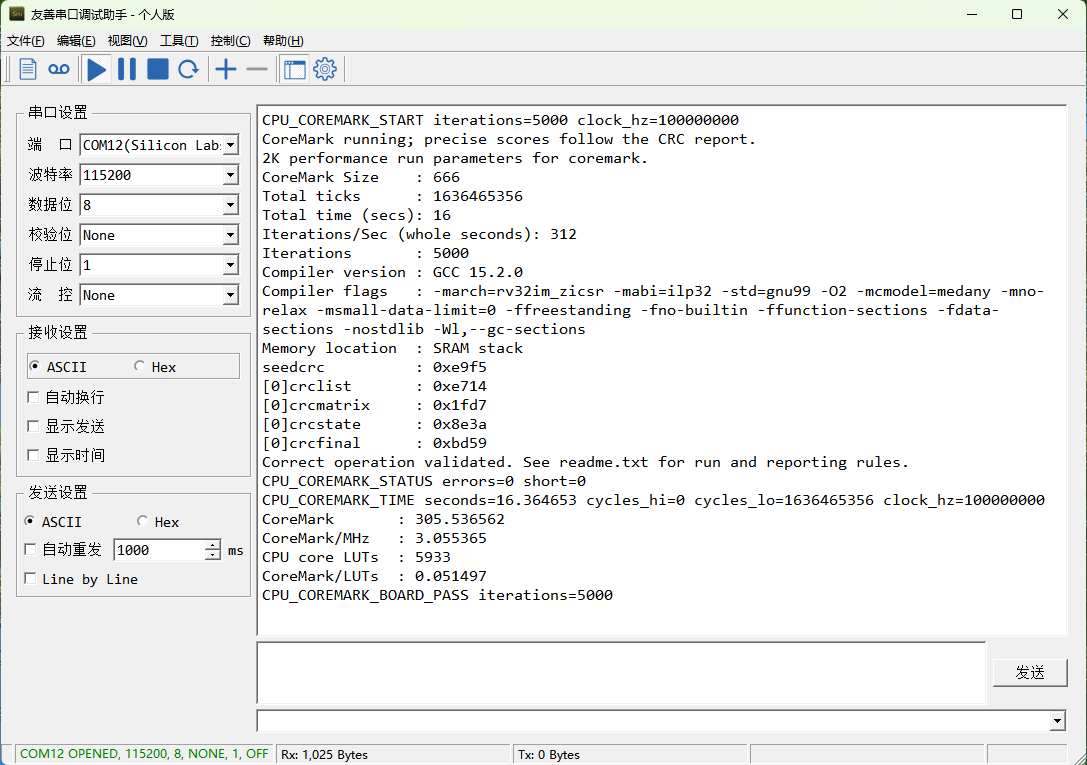
\includegraphics[height=0.34\linewidth]{../figure/cpu-tcm-coremark-uart-original.png}}\hfill
\makebox[0.49\linewidth][c]{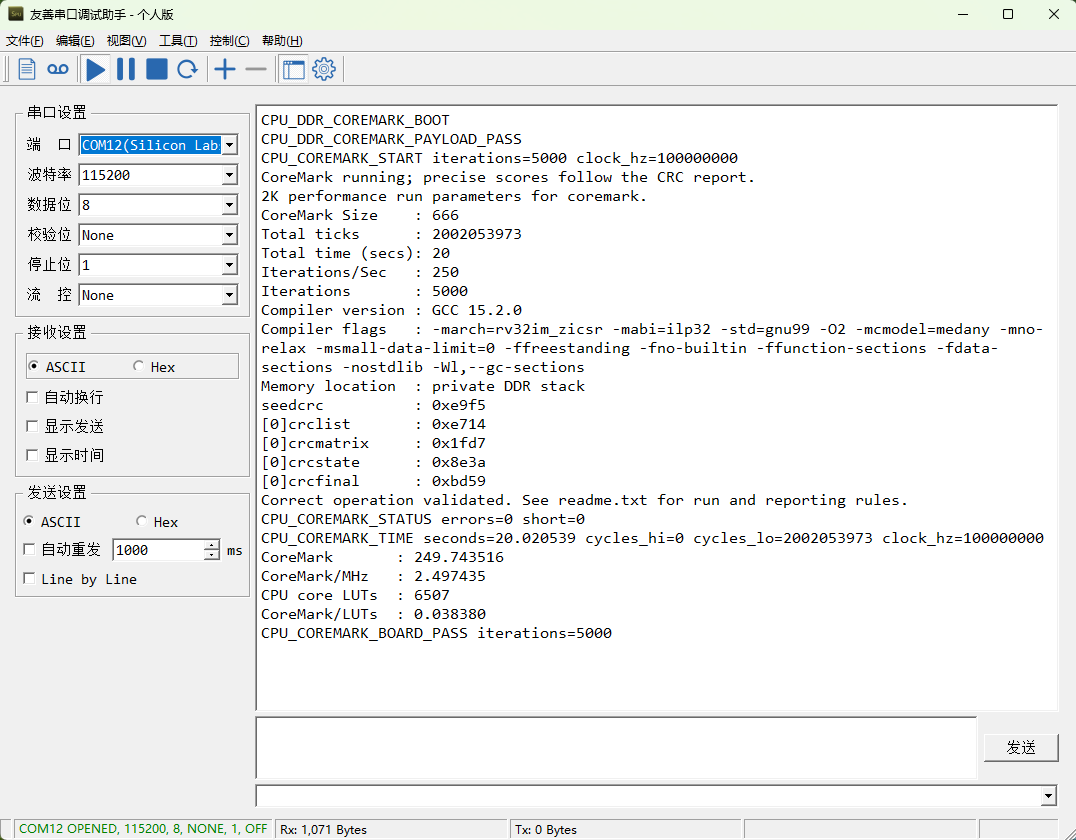
\includegraphics[height=0.34\linewidth]{../figure/cpu-l1-cache-ddr-coremark-uart-original.png}}
\par\smallskip
\makebox[0.49\linewidth][c]{\small (a) 片上SRAM/TCM}\hfill
\makebox[0.49\linewidth][c]{\small (b) L1 Cache＋板载DDR}
\caption{单发射CPU两种存储配置的CoreMark完整串口截图}\label{fig:cpu-single-coremark-uart}
\end{figure}

双发射SRAM与Cache＋DDR的CoreMark/MHz分别比表\ref{tbl:cpu-coremark}中的单发射结果高约33.95\%和26.22\%。
两组板级版本还包含前端、配对和数据通路优化，以上为各自完整配置的结果比较，不将差值全部归因于发射宽度开关。

表\ref{tbl:cpu-resources}按综合报告中的CPU核层级统计资源，片上SRAM、调试核、DDR及板级逻辑均不计入CPU核。
单发射CPU核的688个RAM-LUT和双发射CPU核的752个RAM-LUT均已包含在各自LUT总数中。Cache及传输控制另列，DRM以36\,Kbit块统计。

\begin{reporttable}
\begin{longtable}{@{}p{0.47\linewidth}rrrr@{}}
\caption{CPU核及缓存资源统计}\label{tbl:cpu-resources}\\
\toprule
统计范围 & LUT & FF & DRM & APM \\
\midrule
\endfirsthead
\caption[]{CPU核及缓存资源统计（续）}\\
\toprule
统计范围 & LUT & FF & DRM & APM \\
\midrule
\endhead
\bottomrule
\endfoot
单发射TCM原发布版CPU核 & 5933 & 3528 & 0 & 4 \\
单发射TCM调试版CPU核 & 6139 & 3528 & 0 & 4 \\
单发射Cache＋DDR版CPU核 & 6507 & 3562 & 0 & 4 \\
单发射配置Cache及传输控制 & 668 & 807 & 11 & 0 \\
双发射SRAM版CPU核 & 9677 & 4968 & 0 & 4 \\
双发射Cache＋DDR版CPU核 & 9707 & 4995 & 0 & 4 \\
双发射配置Cache及传输控制 & 675 & 807 & 11 & 0 \\
\end{longtable}
\end{reporttable}

TCM调试版在新综合上下文中得到6139个CPU核LUT，CPU源码和固件与原发布版逐字节相同，板测周期也相同。
原固件在计时结束后仍打印历史5933-LUT元数据；表\ref{tbl:cpu-coremark}使用本次调试构建的6139个LUT重新计算效率。
原无调试核发布包的5933个CPU核LUT和0.051497819 CoreMark/LUT保留为该发布包的结果。

单发射TCM调试版和L1 Cache＋DDR版分别满足100\,MHz实际后布线时序，结果见表\ref{tbl:cpu-board-timing}。
TCM调试版沿用原100\,MHz、I/O延迟及hold约束；四路LED均映射到器件输出寄存器，状态显示延后一拍，退出码组合译码不再直接驱动引脚。
调试核各时钟与跨时钟检查、复位恢复和移除检查均通过，performance slack与最差setup一致。

\begin{reporttable}
\begin{longtable}{@{}p{0.30\linewidth}p{0.30\linewidth}p{0.34\linewidth}@{}}
\caption{单发射CPU板级后布线时序裕量}\label{tbl:cpu-board-timing}\\
\toprule
检查项 & TCM调试版 & L1 Cache＋DDR版 \\
\midrule
\endfirsthead
\caption[]{单发射CPU板级后布线时序裕量（续）}\\
\toprule
检查项 & TCM调试版 & L1 Cache＋DDR版 \\
\midrule
\endhead
\bottomrule
\endfoot
Setup，Slow/Fast & +0.366/+3.662\,ns & +0.309/+3.551\,ns \\
Hold，Slow/Fast & +0.061/+0.034\,ns & +0.151/+0.099\,ns \\
最小脉宽，Slow/Fast & +3.655/+4.202\,ns & +3.655/+4.202\,ns \\
\end{longtable}
\end{reporttable}

双发射两个板级配置也完成100\,MHz后布线时序检查，CPU时钟域结果见表\ref{tbl:cpu-dual-board-timing}。
资源与时序分别取自对应板级构建，Cache＋DDR版的9707个CPU核LUT与串口分母一致，Cache及传输控制的675个LUT单独计数。
双发射提高了单位频率性能，同时增加寄存器读写端口、前递及配对控制的资源开销；按现有板级数据，其CoreMark/LUT低于对应单发射配置。

\begin{reporttable}
\begin{longtable}{@{}p{0.30\linewidth}p{0.30\linewidth}p{0.34\linewidth}@{}}
\caption{双发射CPU板级后布线时序裕量}\label{tbl:cpu-dual-board-timing}\\
\toprule
检查项 & SRAM版 & Cache＋DDR版 \\
\midrule
\endfirsthead
\caption[]{双发射CPU板级后布线时序裕量（续）}\\
\toprule
检查项 & SRAM版 & Cache＋DDR版 \\
\midrule
\endhead
\bottomrule
\endfoot
Setup，Slow/Fast & +0.220/+3.768\,ns & +0.223/+3.447\,ns \\
Hold，Slow/Fast & +0.162/+0.104\,ns & +0.158/+0.102\,ns \\
最小脉宽，Slow/Fast & +3.655/+4.202\,ns & +3.655/+4.202\,ns \\
Recovery，Slow/Fast & +2.036/+4.167\,ns & +4.062/+6.174\,ns \\
Removal，Slow/Fast & +0.653/+0.441\,ns & +0.188/+0.103\,ns \\
\end{longtable}
\end{reporttable}

100\,MHz为这些配置完成时序检查并用于板测的工作点；Fmax需通过对应配置的频率约束扫描确定。
板测CoreMark记录提供运行周期，整段退休IPC另需在同一计时窗口累计两路有效完成指令数。

表\ref{tbl:cpu-issue-tradeoff}按相同存储路径比较两组完整配置，片上路径的单发射分母采用TCM调试版。
双发射在片上SRAM路径增加3538个CPU核LUT，获得33.95\%的CoreMark/MHz提升；在Cache＋DDR路径增加3200个LUT，获得26.22\%的提升。
资源增长快于性能增长，两条路径的CoreMark/LUT分别下降约15.02\%和15.39\%。

\begin{reporttable}
\begin{longtable}{@{}p{0.38\linewidth}p{0.28\linewidth}p{0.28\linewidth}@{}}
\caption{单发射至双发射完整配置的性能与资源变化}\label{tbl:cpu-issue-tradeoff}\\
\toprule
比较项 & 片上SRAM/TCM & L1 Cache＋DDR \\
\midrule
\endfirsthead
\caption[]{单发射至双发射完整配置的性能与资源变化（续）}\\
\toprule
比较项 & 片上SRAM/TCM & L1 Cache＋DDR \\
\midrule
\endhead
\bottomrule
\endfoot
CPU核LUT & 6139 $\rightarrow$ 9677 & 6507 $\rightarrow$ 9707 \\
CPU核LUT增幅 & 57.63\% & 49.18\% \\
CoreMark/MHz增幅 & 33.95\% & 26.22\% \\
CoreMark/LUT变化 & $-15.02\%$ & $-15.39\%$ \\
Slow角Setup裕量 & 0.366 $\rightarrow$ 0.220\,ns & 0.309 $\rightarrow$ 0.223\,ns \\
\end{longtable}
\end{reporttable}

从资源分配看，双发射适合需要提高CPU处理吞吐的配置；单发射在单位LUT性能上更有利，可为NPU和视频缓冲保留更多器件资源。
双发射需要为两条指令提供操作数和独立写回，并扩展操作数前递及配对控制；两种配置均使用4个APM，增加的资源主要体现在LUT和FF。
两组双发射实现均在100\,MHz下保持正的建立、保持裕量，但Slow角建立裕量较对应单发射版本减小，继续提高频率需要重新评估关键路径。
这些比较对应各自的前端、数据通路及物理实现，不能等同于同一版本仅切换\texttt{DUAL\_ISSUE}所得的消融实验。

Cache＋DDR路径的增益较片上路径低，与访存等待限制可并行执行的机会相符。
共享LSU/MUL、指令相关及前端供给共同影响双发射利用率。
本节IPC与周期分类来自单发射数字仿真，测试配置与统计窗口见下文。

\subsection{CPU流水线效率}

片上调试以单发射TCM版本为例，采用PDS DebugCore/Fabric Debugger关联CoreMark函数入口与流水线状态。
调试镜像保留已验收的CPU及5000次\texttt{-O2}固件，仅在板级封装中寄存四路LED输出并加入38位DebugCore探针；实际后布线时序及Program/Verify通过后再进行采样。
该镜像的完整板测周期与无探针发布版一致。采样时钟为CPU时钟上升沿。
三个触发端口分别为30位WB PC\texttt{[31:2]}、1位WB有效和7位流水控制状态，合计38位，采样深度为1024拍。
按32\,bit指令对齐规则在PC低位补零，结合5000次板测ELF定位链表归并排序、矩阵乘法和状态转换的真实函数入口。
触发条件同时要求入口PC匹配、\texttt{valid\_wb\_q=1}和\texttt{pipe0\_stall\_raw\_w=0}。

表\ref{tbl:cpu-sram-kernel-windows}统计完整采样窗口。WB事件按有效位与非暂停状态的交集计数，避免指令保持时重复累加。
窗口可能进入被调函数或调用者；这些局部WB事件不构成整段CoreMark的架构退休IPC，内存WB有效也不等同于DDR事务或Cache事件。

\begin{reporttable}
\begin{longtable}{@{}p{0.24\linewidth}p{0.27\linewidth}rr@{}}
\caption{单发射TCM CPU三个热点的1024拍板上采样}\label{tbl:cpu-sram-kernel-windows}\\
\toprule
触发算法 & 触发PC & WB事件 & 内存WB有效拍 \\
\midrule
\endfirsthead
\caption[]{单发射TCM CPU三个热点的1024拍板上采样（续）}\\
\toprule
触发算法 & 触发PC & WB事件 & 内存WB有效拍 \\
\midrule
\endhead
\bottomrule
\endfoot
链表归并排序 & \texttt{0x00011D48} & 951 & 119 \\
矩阵乘法 & \texttt{0x000124E8} & 964 & 247 \\
状态转换 & \texttt{0x00012C1C} & 916 & 182 \\
\end{longtable}
\end{reporttable}

图\ref{fig:cpu-sram-list-board}、图\ref{fig:cpu-sram-matrix-board}和图\ref{fig:cpu-sram-state-board}为Fabric Debugger最大化窗口的原始采样波形截图，放大展示各入口附近的局部采样。
插图仅裁剪窗口边缘及空白区，保留原始信号名、读值和采样刻度。金色游标0为指定函数入口，对应原始CSV索引1；其前一拍为工具刻度$-1$，对应CSV索引0。
三窗在触发拍均为WB有效且非暂停。\texttt{wb\_pc\_word}为PC[31:2]，游标读值\texttt{0x4752}、\texttt{0x493A}和\texttt{0x4B07}分别对应三个字节地址；PC总线仅在WB事件有效时解释为完成指令地址。
图中\texttt{valid\_e2\_q}表示E2在途状态，\texttt{squash\_e1\_e2\_w}表示取消条件，\texttt{div\_pending\_q}和\texttt{csr\_pending\_q}表示对应串行操作未结束，\texttt{fetch0\_valid\_w}与\texttt{writeback\_mem\_valid\_w}分别表示前端及内存返回有效。
三窗\texttt{pipe0\_stall\_raw\_w}均为零，但\texttt{valid\_wb\_q}仍有空隙；发射空泡、相关性和控制流开销需结合更多前端信号分析，不能只凭该暂停位判断。

\begin{figure}[!htbp]
\centering
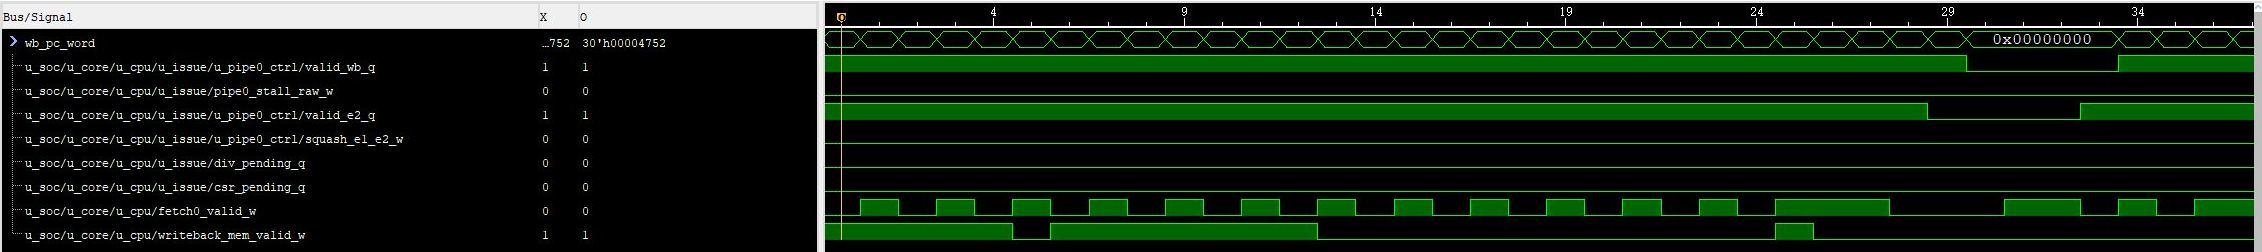
\includegraphics[width=\linewidth]{../figure/cpu-sram-list-native.png}
\caption{单发射TCM CPU链表热点的原始采样截图，触发PC为0x00011D48}\label{fig:cpu-sram-list-board}
\end{figure}

\begin{figure}[!htbp]
\centering
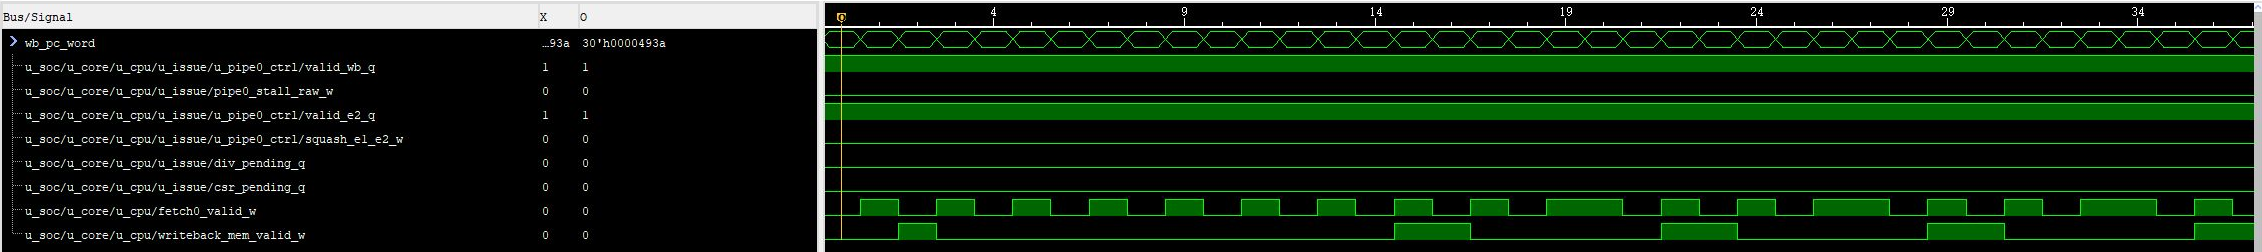
\includegraphics[width=\linewidth]{../figure/cpu-sram-matrix-native.png}
\caption{单发射TCM CPU矩阵热点的原始采样截图，触发PC为0x000124E8}\label{fig:cpu-sram-matrix-board}
\end{figure}

\begin{figure}[!htbp]
\centering
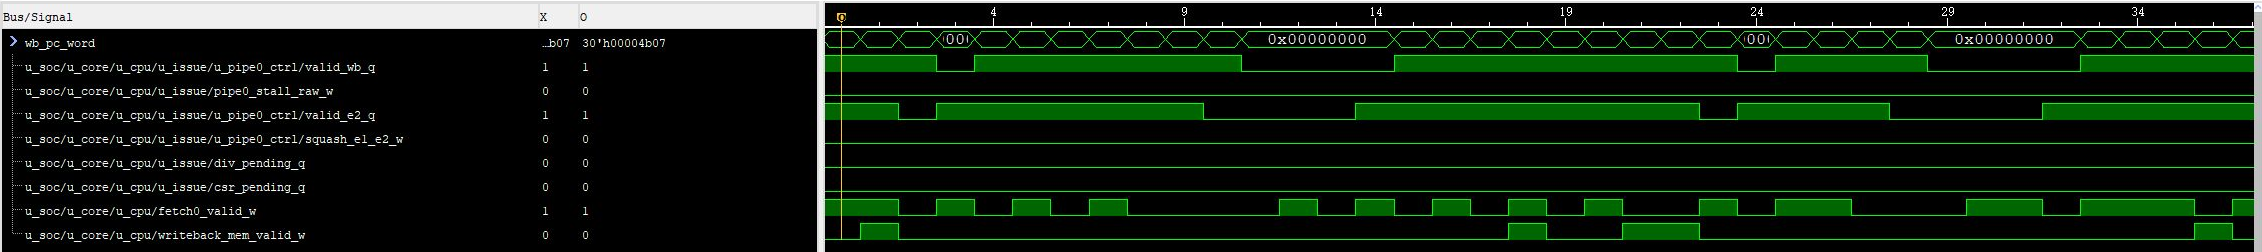
\includegraphics[width=\linewidth]{../figure/cpu-sram-state-native.png}
\caption{单发射TCM CPU状态转换热点的原始采样截图，触发PC为0x00012C1C}\label{fig:cpu-sram-state-board}
\end{figure}

采样归档包含原生DPRJ/WDF、逐拍CSV、触发条件及位流和ELF哈希。
state窗口的38位通道和PC总线在全部1024拍上与原始VCD逐位一致。
原始VCD导出的100\,ns标注属于工具的样本刻度，本节横轴统一使用采样序号；硬件配置的100\,MHz采样时钟名义周期为10\,ns。
上述片上采样属于单发射TCM配置，与对应的单发射完整板测配套；双发射及L1 Cache＋DDR配置分别记录。

单发射Cache/DDR版的整段流水线统计来自ModelSim数字DDR及PLL模型，采用与该版5000次板测CPU/Cache RTL逐字节一致的配置。
软件仍为GCC 15.2、\texttt{-O2}、无LTO，仿真执行5次迭代，UART除数仅在测试台中缩短，计时仍来自CPU周期CSR。
这项短测保留不足10\,s提示，用于分析执行过程。2026年10月28日的观测重放得到2,018,576个计时周期、1,448,453条WB观察序列及70,840次store，标准CRC及完整序列哈希均与原记录一致。
观测模块不驱动CPU、Cache或软件状态。

统计窗口对应软件两次周期CSR读取之间的区间。WB计数包括分支和存储指令，暂停时不重复累加，窗口内异常检查为零。
对应的数字WB观测IPC和CPI为
\begin{equation}
  IPC_{\mathrm{WB}}=\frac{1,448,453}{2,018,576}=0.717562,
  \qquad CPI_{\mathrm{WB}}=1.393608
\end{equation}
该数值为单发射Cache/DDR数字模型的WB观测IPC，其计数范围与板上采样、双发射板测分别记录。

每周期按发射成功、取消、LSU等待、后端流水等待、除法、CSR、前端无有效指令、执行资源、相关性及其他原因的优先顺序归类。
发射成功优先，未发射时取首个阻塞原因；各项互斥且总和等于计时周期数，结果见表\ref{tbl:cpu-cache-cycle-profile}。

\begin{reporttable}
\begin{longtable}{@{}p{0.48\linewidth}rr@{}}
\caption{单发射Cache/DDR数字CoreMark的互斥周期分类}\label{tbl:cpu-cache-cycle-profile}\\
\toprule
周期类别 & 周期数 & 占比（\%） \\
\midrule
\endfirsthead
\caption[]{单发射Cache/DDR数字CoreMark的互斥周期分类（续）}\\
\toprule
周期类别 & 周期数 & 占比（\%） \\
\midrule
\endhead
\bottomrule
\endfoot
发射成功 & 1,448,453 & 71.756179 \\
LSU等待 & 358,437 & 17.756924 \\
后端流水等待 & 12,993 & 0.643672 \\
前端无有效指令 & 98,793 & 4.894193 \\
相关性等待 & 99,891 & 4.948588 \\
CSR等待 & 9 & 0.000446 \\
取消、除法、执行资源及其他类别合计 & 0 & 0.000000 \\
总计 & 2,018,576 & 100.000000 \\
\end{longtable}
\end{reporttable}

该数字窗口中，D-Cache接受273,477次读及70,840次写，读命中273,461次、读未命中16次，读命中率为99.994149\%。
写命中70,824次、写分配未命中16次，共32次行填充；计时窗口内没有脏行逐出或显式清理，下级写次数为零。
高命中率仍伴随17.756924\%的LSU等待，说明请求接纳、同步RAM读取和返回节拍也限制吞吐；成功加载返回与下一请求的重叠发生75,408次。
Cache与总线各状态的周期统计可能包含同一周期，因此不能与上述互斥类别直接相加。

\subsection{NPU性能}

人脸检测应用的NPU采用两空间行Dense阵列和单量化通路，计算时钟为50\,MHz。
CPU提交整帧任务后，图控制器读取NPM3程序，依次执行普通卷积、深度卷积及辅助算子，完成九个检测头的写回。
CPU随后读取这些输出，执行定点解码、NMS和主人脸选择。

框检测部署图的普通及逐点卷积每帧执行68,837,800次MAC，深度卷积执行15,685,200次MAC，总计84,523,000次。
Dense阵列每个有效拍完成$16M$次MAC，DW16每个有效拍完成16次MAC，两条通路按算子分时运行。
在计算频率$f$下，持续有效供数时的纯卷积算术时间下界为
\[
T_{\mathrm{conv,min}}(M,f)=
\frac{68\,837\,800}{16Mf}+\frac{15\,685\,200}{16f}
\]
代入$M=2$、$f=50\times10^6$\,Hz，普通及逐点卷积的理想时间为43.023625\,ms，深度卷积为19.606500\,ms，合计62.630125\,ms。
该下界按持续有效供数和满通路计算，仅计乘加，不包含尾通道及空间块利用率损失、量化、数据搬运、辅助算子、图控制和CPU后处理；组件的数值及时序验证见附录\ref{sec:npu-compute-validation}。
对应的理想纯卷积吞吐上限约为15.97帧/s。24帧/s要求每帧不超过41.667\,ms，已小于普通及逐点卷积单项的理想时间，因此24帧/s属于后续优化目标，当前50\,MHz、$M=2$配置即使忽略其他开销也无法达到。

完整应用仿真采用与上板版本一致的计算、Video和像素时钟，运行实际CPU固件、NPU、Video及跨域逻辑，外存端点采用存储代理模型。
输入经过视频采集与预处理后进入NPU，计算结果由CPU后处理，并形成同帧显示记录。
统计以CPU后处理结果完成事件为边界，数值列于表\ref{tbl:face-result-intervals}。

\subsection{系统性能}

系统分别记录结果完成、显示记录生效和实际像素输出。
表\ref{tbl:face-result-intervals}给出50\,MHz应用仿真的两组结果间隔。
自然人脸与零RGB空场景各运行至两个结果完成，每组取相邻完成事件之间的一个间隔样本。

\begin{reporttable}
\small
\begin{longtable}{@{}lrrr@{}}
\caption{整帧应用仿真的结果完成间隔}\label{tbl:face-result-intervals}\\
\toprule
场景 & 间隔（计算周期） & 间隔（ms） & 结果速率（fps） \\
\midrule
\endfirsthead
\caption[]{整帧应用仿真的结果完成间隔（续）}\\
\toprule
场景 & 间隔（计算周期） & 间隔（ms） & 结果速率（fps） \\
\midrule
\endhead
\bottomrule
\endfoot
自然人脸 & 18079060 & 361.58120 & 2.76563 \\
零RGB空场景 & 18060318 & 361.20636 & 2.76850 \\
\end{longtable}
\end{reporttable}

自然人脸的结果完成标记为第22,023,646和40,102,706个计算周期，零RGB空场景为第21,998,338和40,058,656个计算周期。
间隔与结果完成率按下式计算，其中$C_1$、$C_2$为两个事件的计算周期计数：
\[
\Delta t=\frac{C_2-C_1}{50\times10^6},\qquad
r_{\mathrm{result}}=\frac{50\times10^6}{C_2-C_1}
\]
日志标记\texttt{FACE\_SYSTEM\_NPU\_CPU\_RESULT}由软件\texttt{results}计数增加触发，位于CPU后处理、显示记录构建及NPU完成确认之后。
相邻事件间隔覆盖逐帧预检、图执行、数据访问、CPU后处理及调度等待；一次性模型及头像装载和启动位于首个事件之前，不计入该间隔。
两组结果反映给定存储代理环境中的结果生成率，每场景只有一个间隔样本，不能作为板级持续帧率。

两个间隔分别为纯卷积算术下界的5.7733倍和5.7673倍，相差298.9511\,ms和298.5762\,ms。
差额混合了实际计算利用率损失及公式未计入的系统工作，不能全部归为访存或调度开销，也不能据此反推PE实测利用率。
现有日志每十个算子记录一次完成检查点。第二帧的\texttt{op0}至\texttt{op10}完成间隔分别为163.47200\,ms和163.48584\,ms，表明该区间是后续剖析的重点；其中包含\texttt{op1}至\texttt{op10}的混合算子、访存及层间等待。
\texttt{op70}至结果完成之间还包括末尾八个算子、图退出和CPU处理，不能直接作为CPU后处理耗时。
表\ref{tbl:system-profile-evidence}列出分项分析可用的证据与缺失观察量。

\begin{reporttable}
\small
\begin{longtable}{@{}p{0.16\linewidth}p{0.34\linewidth}p{0.43\linewidth}@{}}
\caption{整机耗时分析的证据与缺失观察量}\label{tbl:system-profile-evidence}\\
\toprule
分项 & 已有证据 & 分解实测耗时所需记录 \\
\midrule
\endfirsthead
\caption[]{整机耗时分析的证据与缺失观察量（续）}\\
\toprule
分项 & 已有证据 & 分解实测耗时所需记录 \\
\midrule
\endhead
\bottomrule
\endfoot
Dense & 算子形状及32\,MAC/周期理想峰值 & 逐算子起止、有效计算与停顿周期 \\
DW & 16路通路及量化握手 & 逐算子起止、有效输入输出与阻塞周期 \\
量化 & 单量化通路配置 & 请求、完成和反压周期，与计算的重叠范围 \\
辅助算子 & 32个非卷积算子及稀疏完成点 & 各算子类型的完整执行区间 \\
DMA及回写 & 累计读写事务数 & 按帧及请求方记录字节数、首末响应与等待 \\
图控制 & 逐帧预检和阶段／算子状态 & 预检、执行、层间等待的起止及重叠关系 \\
CPU后处理 & 结果完成事件位于后处理之后 & 输出头收取、解码／NMS、记录构建及ACK的独立起止 \\
\end{longtable}
\end{reporttable}

上述通路可以重叠工作，各自忙周期不能直接相加为总时间。现有正式日志没有完整的分项边界，因此不列各模块耗时比例。

有效输出帧率以统计窗口内首次实际显示的不同采集帧数计数。
同一帧的重复扫描不增加新帧数；采集、结果完成与显示扫描使用各自事件标记，不能互相替代。
板内可见延迟的起点为选中输入帧的有效画面开始，终点为全屏输出首次显示该帧结果的有效像素。
表\ref{tbl:system-latency-boundaries}列出各阶段的事件边界。
其中\texttt{RESULT\_READY}表示上述应用软件结果完成边界，不指代单独的NPU完成脉冲。

\begin{reporttable}
\begin{longtable}{@{}p{0.22\linewidth}>{\raggedright\arraybackslash}p{0.37\linewidth}p{0.35\linewidth}@{}}
\caption{系统处理与显示延迟的统计边界}\label{tbl:system-latency-boundaries}\\
\toprule
阶段 & 起止事件 & 计入内容 \\
\midrule
\endfirsthead
\caption[]{系统处理与显示延迟的统计边界（续）}\\
\toprule
阶段 & 起止事件 & 计入内容 \\
\midrule
\endhead
\bottomrule
\endfoot
输入形成 & 输入首个有效像素至\texttt{INPUT\_READY} & 采集、预处理、DDR写入及响应排空 \\
推理与后处理 & \texttt{INPUT\_READY}至\texttt{RESULT\_READY} & 调度等待、NPU图执行、计算与搬运、CPU后处理 \\
显示等待 & \texttt{RESULT\_READY}至匹配显示记录的SOF & 提交握手与帧边界等待 \\
像素生效 & 记录生效SOF至首个对应有效像素实际输出 & 原图读取、框或头像合成及输出流水 \\
有效输出吞吐 & 相邻新帧首次实际显示事件 & 不同采集帧的更新间隔 \\
\end{longtable}
\end{reporttable}

40\,MHz像素时钟和$1056\times628$扫描总时序对应约60.31654\,Hz，扫描周期为16.5792\,ms。
当显示记录和原图数据就绪、下一帧边界可以接纳时，等待SOF的时间处于一个扫描周期内；SOF后的像素输出还经过读取和合成流水。
该扫描参数用于解释显示时序，相邻检测结果的完成间隔按上表的独立事件统计。
板测记录确认了三模式切换、头像跟随、透明合成和无脸清除与恢复，但没有保存同一采样窗口内的结果完成数、新采集帧首次显示数及扫描数，实际板级结果完成率和新图更新率尚未测得。
后续测量需在同一会话内记录起止时间及对应计数，同时核对帧身份、仅模式切换事件、拒绝、欠载和错误；软件无空闲槽的尝试次数不等于输入丢帧数。
本节仿真、板级功能验收及原始日志统一归档于\path{docs/verification/soc/face_photo_report_20261104/}。

\subsection{FPGA实现指标}

人脸检测整机在PG2L100H-6IFBG676上完成综合和布局布线，综合总数为45,716个LUT、41,848个FF、113.5个DRM36K等效块和64个APM。
按器件容量折算分别为68.64\%、31.42\%、73.23\%和26.67\%；同一构建的模块层级资源见表\ref{tbl:board-resources}。
CPU与NPU工作于50\,MHz，Video与DDR用户接口工作于125\,MHz，输出像素时钟为40\,MHz。

表\ref{tbl:face-board-timing}列出最终布线数据库的内部时序检查结果，所有列示检查的失败端点数均为0。

\begin{reporttable}
\begin{longtable}{@{}lrr@{}}
\caption{人脸检测整机内部后布线时序裕量}\label{tbl:face-board-timing}\\
\toprule
检查项 & Slow（ns） & Fast（ns） \\
\midrule
\endfirsthead
\caption[]{人脸检测整机内部后布线时序裕量（续）}\\
\toprule
检查项 & Slow（ns） & Fast（ns） \\
\midrule
\endhead
\bottomrule
\endfoot
建立时间 & +0.100 & +2.891 \\
保持时间 & +0.187 & +0.131 \\
恢复时间 & +2.066 & +4.089 \\
移除时间 & +0.314 & +0.206 \\
最小脉宽 & +0.035 & +0.035 \\
\end{longtable}
\end{reporttable}

Slow角的计算时钟域建立裕量为+2.287\,ns，DDR用户时钟域为+0.100\,ns，输出像素时钟域为+9.406\,ns。
CDC检查覆盖23组、116个Gray指针位及928次源、目的时钟观测，最大保守到达偏差界为3.479\,ns，各组均满足各自约束。
这些结果对应冻结布线数据库中的内部路径与跨域约束，工作频率按该构建的实际时钟列示。

表\ref{tbl:board-critical-setup}列出一条最差建立路径，位于模型输入采集DMA的基址及描述符校验逻辑中，经过10级组合逻辑。
报告起点为\texttt{dma\_\allowbreak base\_\allowbreak reg[14]}的CLK端，对应首个数据弧为\texttt{dma\_\allowbreak base\_\allowbreak reg[12]}的Q端，终点为\texttt{row\_\allowbreak base[22]}的时钟使能端；这些名称按综合后报告保留。
该路径属于125\,MHz DDR用户时钟域，至行基址寄存器第24、26、28位的路径具有相同的最差裕量。

\begin{reporttable}
\begin{longtable}{@{}p{0.35\linewidth}p{0.58\linewidth}@{}}
\caption{整机Slow角最差建立路径}\label{tbl:board-critical-setup}\\
\toprule
项目 & 报告值 \\
\midrule
\endfirsthead
\caption[]{整机Slow角最差建立路径（续）}\\
\toprule
项目 & 报告值 \\
\midrule
\endhead
\bottomrule
\endfoot
发起／接收时钟 & \texttt{ddrphy\_sysclk}，125\,MHz，周期8.000\,ns \\
组合逻辑级数 & 10 \\
逻辑／布线延迟 & 1.734／5.335\,ns，逻辑项含时钟到Q延迟 \\
总数据路径延迟 & 7.069\,ns \\
有效时钟偏差 & $-0.255$\,ns，已计时钟悲观量移除 \\
不确定度／建立时间 & 0.350／0.226\,ns，采用报告实际计入值 \\
数据到达／要求时间 & 12.640／12.740\,ns \\
建立裕量 & $12.740-12.640=+0.100$\,ns \\
\end{longtable}
\end{reporttable}

布线占该路径数据延迟的75.47\%，说明此路径的时序主要受布局与连线影响；该比例只描述此条路径，不是整机运行时间占比。
外部DDR PHY和HDMI I/O的板级AC验收与上述内部STA结果分别管理。

